\section{Future Work}
\label{sec:future_work}

In future work, we will extend our experiments from NSD Subjects 1 and 2 to the full four-subject setting used by other papers. This would evaluate whether the observed performance of our pipeline holds up across subjects with differing brain anatomies.

We would likely implement this by introducing a functional clustering space shared across subjects. Specifically, we would summarize each flatmap patch across trials into a single descriptor vector, then fit a Gaussian Mixture Model \cite{dempster1977maximum} to map brain patches from all subjects into a common cluster space. A cross-attention layer could then compress the patches assigned to each cluster into a fixed set of cluster tokens. Similar strategies have proven effective in prior work for training a single transferable model across many subjects \cite{beliy2026wisdomcrowdbrainsuniversal, beliy2025brainitimagereconstructionfmri}.

Together, these extensions would enable a more direct comparison against prior multi-subject methods and test whether our approach remains competitive at scale.

Another direction is to replace CLIP as the target semantic representation with the embedding space of a more recent model such as SigLIP2 \cite{tschannen2025siglip2multilingualvisionlanguage}. One limitation of our current pipeline is that semantic conditioning on CLIP embeddings comes at the expense of low-level performance. Replacing CLIP with a stronger semantic embedding model such as SigLIP2 could improve visual-semantic alignment and, in turn, performance on both low-level and high-level evaluations. This may require training an SDXL decoder that accepts SigLIP2 embeddings as conditioning inputs.

\begin{figure}[!t]
\centering
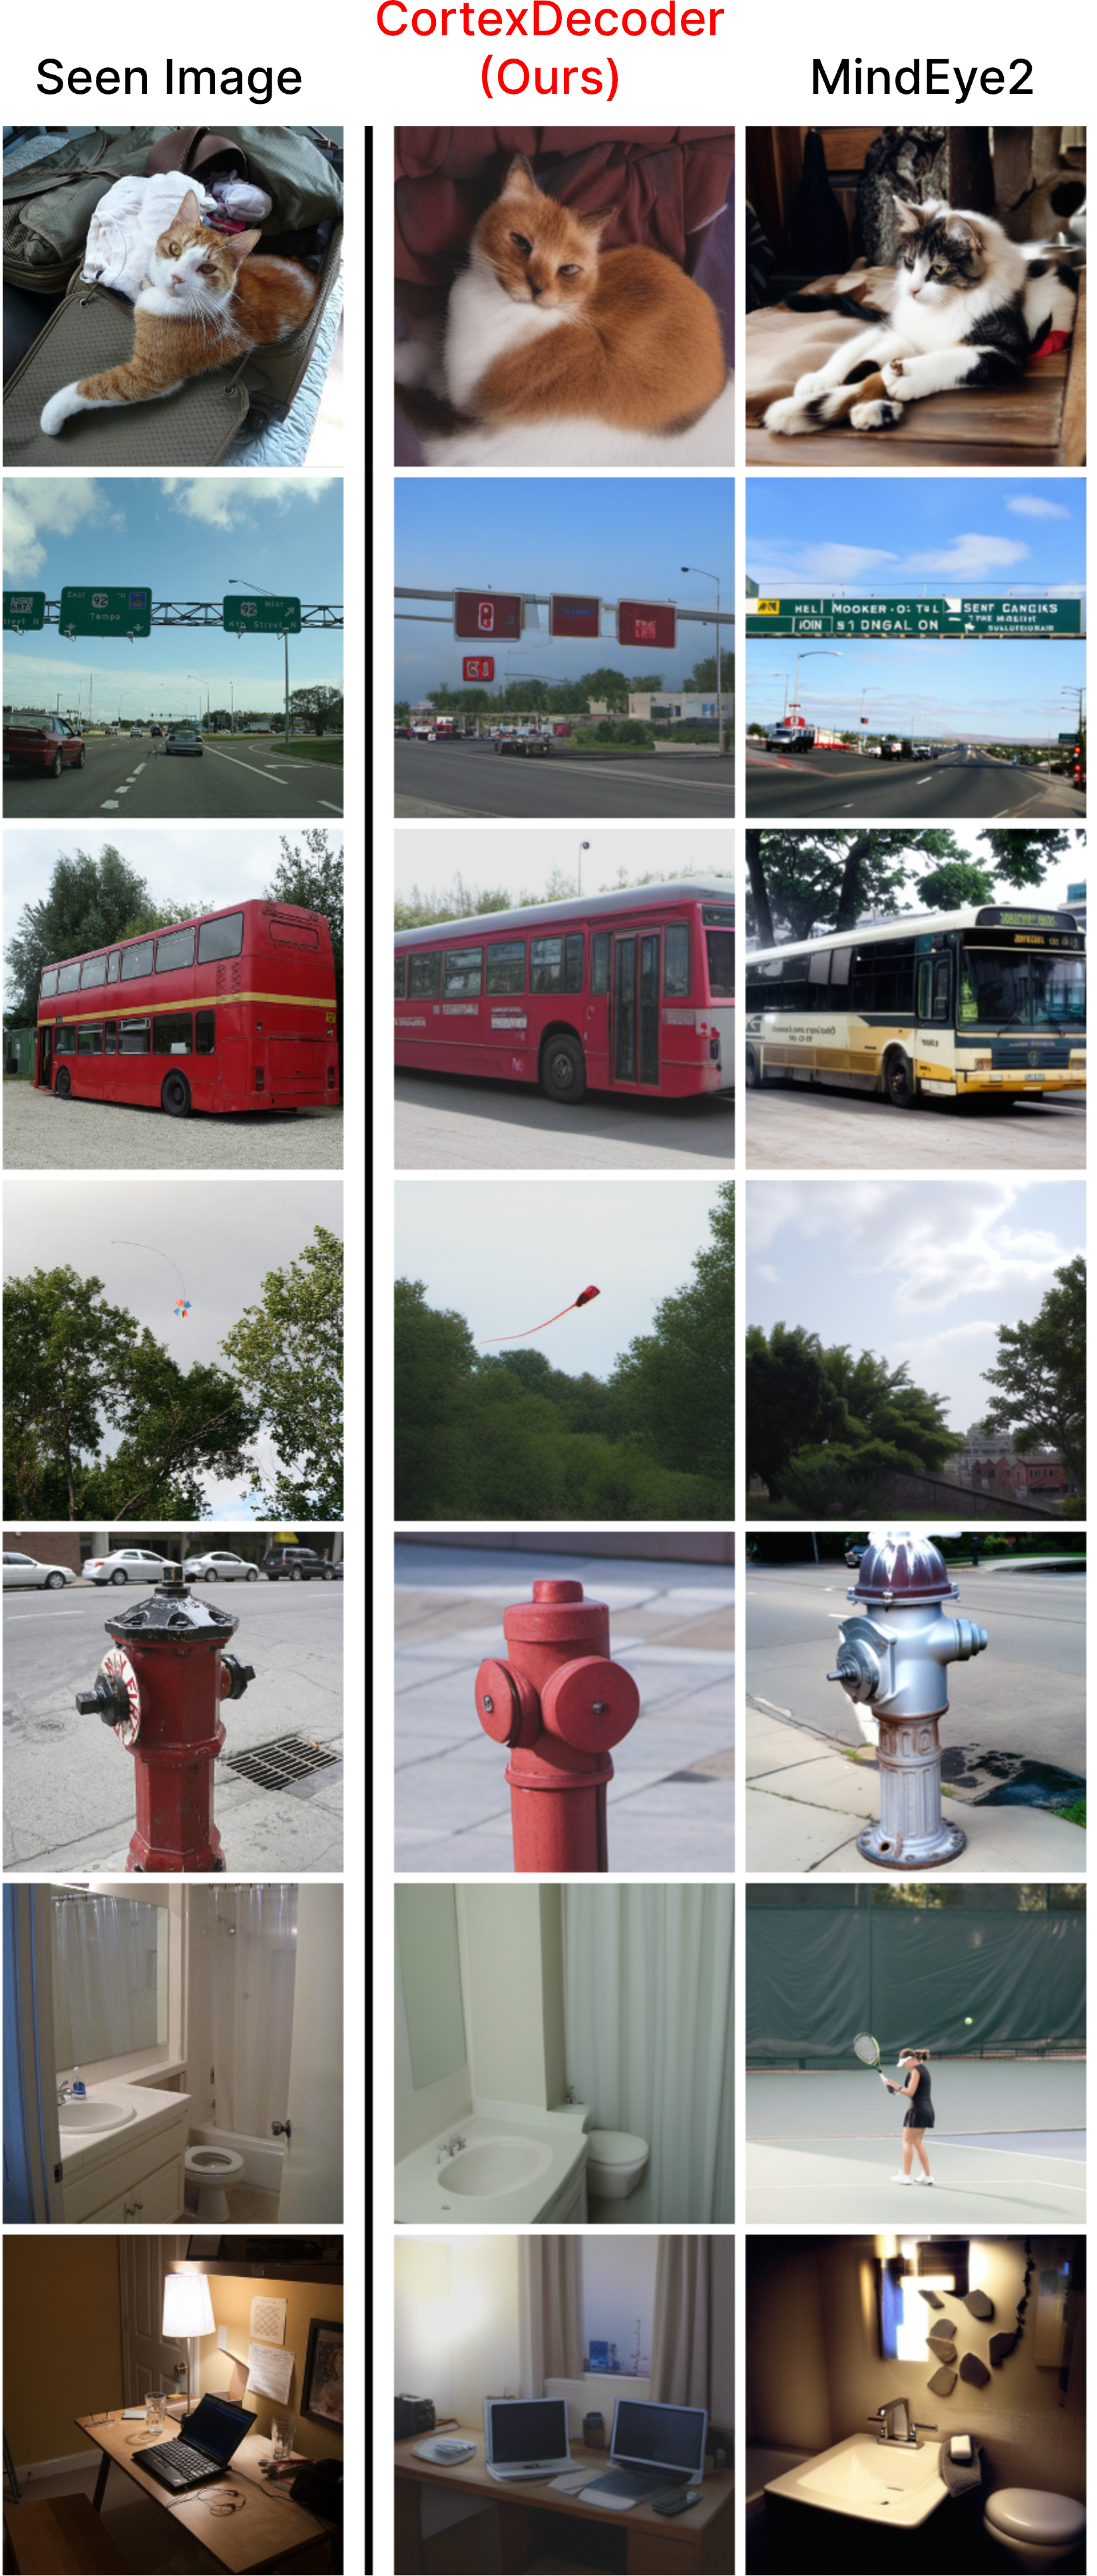
\includegraphics[width=0.8\columnwidth]{images/comparison4.png}
\caption{Stimulus (left), CortexDecoder (middle) and MindEye2 (right) reconstructions. Images from COCO \cite{lin2015microsoftcococommonobjects} (CC BY 4.0).}
\label{fig:comparison}
\end{figure}
